\documentclass[12pt]{article}

\usepackage{latexsym}
\usepackage{amsfonts}
\usepackage{amsmath, amsthm, amssymb}
\usepackage{graphicx}
\usepackage{hyperref}
\usepackage{sectsty}

\usepackage{color}
\usepackage{hyperref}

\hypersetup{
    colorlinks=true, % set true if you want colored links
    linktoc=all,     % set to all if you want both sections and subsections linked
    linkcolor=blue,  % choose some color if you want links to stand out
}

\setlength{\textheight}{10in}
\setlength{\textwidth}{6.5in}
\setlength{\topmargin}{-1.0in}
\setlength{\parskip}{0.15in}
\setlength{\oddsidemargin}{-0.1in}

\sectionfont{\fontsize{10}{10}\selectfont}
\subsectionfont{\fontsize{10}{10}\selectfont}

\newcommand{\DS} [1] {${\displaystyle #1}$}
\renewcommand{\thesubsection}{\thesection.\alph{subsection}}

\author{Michael Walker}
\title{Math 2311 $-$ Assignment 1}
\date{\today}

\begin{document}
\maketitle
\tableofcontents
\pagebreak
\section{Determine if each of the following sets is a vector space.}
\begin{enumerate}
        \item[1.a]Question: $V=$\DS{ \left\{ \left[ \begin{array}{c}
                                      x \\
                                      y
                              \end{array} \right] \in\mathbb{R}^2 \ | \ x \geq{y} \right\}}
              with the usual scalar multiplication
              and vector addition from $\mathbb{R}^2$
\end{enumerate}
\subsection{Answer: No, $V$ is not a vector space.}

\begin{proof}
        Counter example Axiom 5 fails.
        \begin{align*}
                (3, 2) \in S      & : 3\geq 2 \\
                (-3, -2) \notin S & : -3 < -2
        \end{align*}
        For $V$ to be a vector space, all 10 of our vector space axioms must hold; this means it is enough to demonstrate one axiom fails; we have shown $\exists\ \vec{u} \in V: -\vec{u} \notin V$, therefore, $V$ is not a vector space.
\end{proof}
\begin{enumerate}
        \item[1.b]Question: Consider the set $W = \{f \in F(-\infty, \infty) \ | f(1) = 0\}$
              with the usual scalar multiplication and vector addition from
              $F(-\infty, \infty)$.
              Is $W$ a vector space?
\end{enumerate}
\subsection{Answer: Yes, $W$ is a vector space.}
\begin{proof}
        Since we know that $F(-\infty, \infty)$ (with the usual operations) is a vector space,
        and since $W$ is a subset of $F(-\infty, \infty)$ (with the same operations),
        it suffices to prove that $W$ is a subspace of $F(-\infty, \infty)$. To this end we must show three things.\\

        (1) Prove that $W$ is non-empty.\\
        Clearly the zero function ($\mathbf{0})(1)=f(1)=0\therefore W$ is non-empty.\\

        (2) Prove that $W$ is closed under addition.\\
        Let $g \in W$. We must show that $f+g \in W$.
        \begin{align*}
                (f+g)(1) & = f(1) + g(1) & \textrm{(definition of addition of functions)} \\
                         & = 0           & \textrm{($f$ and $g$ are in $W$)}
        \end{align*}

        (3) Prove that $W$ is closed under scalar multiplication. \\
        Let scalar $k \in \Re $, then
        \begin{align*}
                (kf)(1) & = kf(1) & \textrm{(definition of scalar multiplication on functions)} \\
                        & = 0     & \textrm{($f$ is in $W$)}
        \end{align*}
        so $W$ is closed under scalar multiplication.\\

        Therefore $W$ is a subspace of $F(-\infty, \infty)$ and hence is a vector space.
\end{proof}
\pagebreak
\section{Let $V$ be a vector space.}
\begin{enumerate}
        \item [2.a]Question: If $k$ is any scalar, prove that $k\vec{0} = \vec{0}$.
\end{enumerate}
\subsection[Proof: $k\vec{0} = \vec{0}$]{}
\begin{proof}
        \begin{align*}
                k\vec{0}             & = k(\vec{0} + \vec{0})                & \textrm{($\vec{0} = \vec{0}+\vec{0}$ by axiom 4)} \\
                                     & = k\vec{0} + k\vec{0}                 & \textrm{(by axiom 7)}                             \\
                k\vec{0}+(-k\vec{0}) & = [k\vec{0} + k\vec{0}] + (-k\vec{0}) & \textrm{(by axiom 5 $k\vec{0}$ has a negative)}   \\
                k\vec{0}+(-k\vec{0}) & = k\vec{0} + [k\vec{0} + (-k\vec{0})] & \textrm{(by axiom 3)}                             \\
                \vec{0}              & = \vec{0} + k\vec{0}                  & \textrm{(by axiom 5)}                             \\
                \vec{0}              & = k\vec{0}                            & \textrm{(by axiom 4)}
        \end{align*}
\end{proof}
\begin{enumerate}
        \item[2.b]Question: Prove that the zero vector in $V$ is unique.
\end{enumerate}
\subsection[Proof: the zero vector in $V$ is unique]{}
\begin{proof}
        We must show that there is only one vector, $\vec{0}$, with the property that \\
        $\vec{0} + \vec{v} = \vec{v} + \vec{0} = \vec{v}$.

        Suppose $\vec{0_1}$ and $\vec{0}$ are zero vectors in $V$ Then $\vec{v} + \vec{0} = \vec{v}\ \land \vec{v} + \vec{0_1} = \vec{v}$
        \begin{align*}
                \vec{0_1} & = \vec{0_1} + \vec{0} & \textrm{(vector space axiom 4)} \\
                          & = \vec{0} + \vec{0_1} & \textrm{(vector space axiom 2)} \\
                          & = \vec{0}             & \textrm{(vector space axiom 4)}
        \end{align*}
        Therefore $\vec{0_1} = \vec{0}$. So, the zero vector is unique.
\end{proof}
\pagebreak
\section{Determine if each of the following are subspaces of $M_{nn}$}
\begin{enumerate}
        \item [3.a]Question: \DS{ \left\{A\in{M_{nn}} \ | det (A) = 0 \right\}}
\end{enumerate}
\subsection{Answer: No, $W$ is not a subspace of $M_{nn}$.}
\begin{proof}
        Counter example Axiom 1 fails \\
        \begin{equation*}
                \det
                \begin{vmatrix}
                        {1} & {0} \\
                        {0} & {0} \\
                \end{vmatrix}
                {= 0},
                \det
                \begin{vmatrix}
                        {0} & {0} \\
                        {0} & {1} \\
                \end{vmatrix}
                = 0
        \end{equation*}
        \begin{equation*}
                \begin{bmatrix}
                        {1} & {0} \\
                        {0} & {0} \\
                \end{bmatrix}
                +
                \begin{bmatrix}
                        {0} & {0} \\
                        {0} & {1} \\
                \end{bmatrix}
                =
                \begin{bmatrix}
                        {1} & {0} \\
                        {0} & {1} \\
                \end{bmatrix}
        \end{equation*}
        \begin{equation*}
                \det
                \begin{vmatrix}
                        {1} & {0} \\
                        {0} & {1} \\
                \end{vmatrix}
                = 1 \neq 0
        \end{equation*}
        A subset $W$ of $M_{nn}$ is a subspace of $M_{nn}$ if and only if
        $W$ satisfies the following three conditions $W$ is nonempty,
        $W$ is closed under addition, $W$ is closed under scalar multiplication.
        We have shown $W$ is not closed under addition; therefore, $W$ is not a subspace of $M_{nn}$.
\end{proof}
\begin{enumerate}
        \item[3.b]Question: \DS{ \left\{A \in{M_{nn}} \ | tr (A) = 0 \right\}}
\end{enumerate}
\subsection{Answer: Yes, $W$ is a subspace of $M_{nn}$}
\begin{proof}
        To prove that $W$ is a subspace of $M_{nn}$ we must show three things.\\\\
        (1) Prove that $W$ is non empty.
        \begin{align*}
                A=({a_{ij})=0}\ \forall\ ij \implies tr(A)=0 \therefore \vec{0} \in W
        \end{align*}
        (2) Prove that $W$ is closed under addition.

        Let $A = ({a_{ii}})\land B = ({b_{ii}})\in W$ be square matricies of order n such that $tr(A) = tr(B) = 0$
        \begin{align*}
                tr(A+B)             & = \sum_{i = 1}^{n}(a_{ii}+b_{ii}) = \sum_{i = 1}^{n}a_{ii} + \sum_{i = 1}^{n}b_{ii} \\
                                    & = tr(A) + tr(B) = 0 + 0 = 0                                                         \\
                \implies C\in W : C & = A+B
        \end{align*}
        (3) Prove that $W$ is closed under multiplication.

        Let ${k}$ be any scalar.
        \begin{align*}
                tr(kA)      & = \sum_{i = 1}^{n}(k\cdot a_{ii}) = k\cdot \sum_{i = 1}^{n}a_{ii} \\
                            & = k\cdot tr(A) = k\cdot 0 = 0                                     \\
                \implies kA & \in W
        \end{align*}
        $\therefore W$ is a subspace of $M_{nn}$.
\end{proof}
\pagebreak
\begin{enumerate}
        \item [3.c]Question: \DS{ \left\{A \in{M_{nn}} \ | A^T = A \right\}}
\end{enumerate}
\subsection{Answer: Yes, $W$ is a subspace of $M_{nn}$}
\begin{proof}
        To prove that $W$ is a subspace of $M_{nn}$ we must show three things.\\\\
        (1) Prove that $W$ is non empty.
        \begin{align*}
                A=({a_{ij})=0}\ \forall\ ij \implies A = A^{T}=0 \therefore \vec{0} \in W
        \end{align*}
        (2) Prove that $W$ is closed under addition.

        Let $A = ({a_{ii}})\land B = ({b_{ii}})\in W$ be square matricies of order n such that $a_{ij}=a{ji}\land b_{ij} = b_{ji}$\
        \begin{align*}
                (A+B)^T             & = A^T+B^T \\
                                    & = A + B   \\
                \implies C\in W : C & = A+B
        \end{align*}
        (3) Prove that $W$ is closed under multiplication.

        Let ${k}$ be any scalar.
        \begin{align*}
                (k\cdot A)^{T} & = k\cdot A^{T} \\
                               & = k\cdot A     \\
                \implies kA    & \in W
        \end{align*}
        $\therefore W$ is a subspace of $M_{nn}$.
\end{proof} \pagebreak
\section{Consider the following vectors in $P_2$: $\vec{p_1} = 2 + x + 4x^2$, $\vec{p_2} = 1 - x + 3x^2$, $\vec{p_3} = 3 + 2x + 5x^2$}
\begin{enumerate}
        \item[4.a]Question: Express the vector $\vec{g} = 6 + 11x + 6x^2$ as a linear combination of $\{\vec{p_1},\vec{p_2},\vec{p_3}\}$.
\end{enumerate}
\subsection{Answer: $\vec{g} =  4(2 + x + 4x^2) +  -5(1 - x + 3x^2) +  1(3 + 2x + 5x^2)$}
\begin{proof} We will show $\vec{g} = k_{1}\vec{p_{1}} + k_{2}\vec{p_{2}} + k_{3}\vec{p_{3}}$
        \begin{align*}
                (6 + 11x + 6x^2) & =  k_{1}(2 + x + 4x^2) +  k_{2}(1 - x + 3x^2) +  k_{3}(3 + 2x + 5x^2)                                \\
                                 & =  (k_{1}2 + k_{2} + k_{3}3)  +  (k_{1}x - k_{2}x + k_{3}2x)  +  (k_{1}4x^2 + k_{2}3x^2 + k_{3}5x^2) \\
                                 & =  (k_{1}2 + k_{2} + k_{3}3)  +  (k_{1} - k_{2} + k_{3}2)x    +  (k_{1}4 + k_{2}3 + k_{3}5)x^2
        \end{align*}
        \begin{align*}
                 &
                \begin{bmatrix}
                        2 & 1  & 3 & \bigm| & 6  \\
                        1 & -1 & 2 & \bigm| & 11 \\
                        4 & 3  & 5 & \bigm| & 6  \\
                \end{bmatrix} \\
                [-2r2+r1] \wedge [-4r2+r1]
                 &
                \begin{bmatrix}
                        0 & 3  & -1 & \bigm| & -16 \\
                        1 & -1 & 2  & \bigm| & 11  \\
                        0 & 7  & -3 & \bigm| & -38 \\
                \end{bmatrix} \\
                r2\leftrightarrow r1
                 &
                \begin{bmatrix}
                        1 & -1 & 2  & \bigm| & 11  \\
                        0 & 3  & -1 & \bigm| & -16 \\
                        0 & 7  & -3 & \bigm| & -38 \\
                \end{bmatrix} \\
                \frac{1}{3}r2
                 &
                \begin{bmatrix}
                        1 & -1 & 2            & \bigm| & 11            \\
                        0 & 1  & \frac{-1}{3} & \bigm| & \frac{-16}{3} \\
                        0 & 7  & -3           & \bigm| & -38           \\
                \end{bmatrix} \\
                -7r2+r3
                 &
                \begin{bmatrix}
                        1 & -1 & 2            & \bigm| & 11            \\
                        0 & 1  & \frac{-1}{3} & \bigm| & \frac{-16}{3} \\
                        0 & 0  & \frac{-2}{3} & \bigm| & \frac{-2}{3}  \\
                \end{bmatrix} \\
                -\frac{3}{2}r3
                 &
                \begin{bmatrix}
                        1 & -1 & 2            & \bigm| & 11            \\
                        0 & 1  & \frac{-1}{3} & \bigm| & \frac{-16}{3} \\
                        0 & 0  & 1            & \bigm| & 1             \\
                \end{bmatrix} \\
                \frac{1}{3}r3+r2
                 &
                \begin{bmatrix}
                        1 & -1 & 2 & \bigm| & 11 \\
                        0 & 1  & 0 & \bigm| & -5 \\
                        0 & 0  & 1 & \bigm| & 1  \\
                \end{bmatrix} \\
                r1 + r2
                 &
                \begin{bmatrix}
                        1 & 0 & 2 & \bigm| & 6  \\
                        0 & 1 & 0 & \bigm| & -5 \\
                        0 & 0 & 1 & \bigm| & 1  \\
                \end{bmatrix} \\
                r1 + r3
                 &
                \begin{bmatrix}
                        1 & 0 & 0 & \bigm| & 4  \\
                        0 & 1 & 0 & \bigm| & -5 \\
                        0 & 0 & 1 & \bigm| & 1  \\
                \end{bmatrix} \\
                \implies (k_{1}, k_{2}, k_{3}) = (4, -5, 1)
        \end{align*}
        $\therefore \vec{g}$ can be expressed as the following linear combination $\vec{g} = k_{1}\vec{p_{1}} + k_{2}\vec{p_{2}} + k_{3}\vec{p_{3}}$
\end{proof}
\pagebreak
\begin{enumerate}
        \item[4.b]Question: Does $\{\vec{p_1},\vec{p_2},\vec{p_3}\}$ span $P_2$?
\end{enumerate}
\subsection{Answer: Yes, $span(\{\vec{p_{1}},\vec{p_{2}},\vec{p_{3}}\}) = P_{2}$}
\begin{proof}
        An arbitrary vector in $P_{2}$ is of the form $\vec{p}=a+bx+cx^2$ and so becomes,\\\\
        $k_{0}(2 + x + 4x^2) +  k_{1}(1 - x + 3x^2) + k_{2}(3 + 2x + 5x^2) = a+bx+cx^2$\\\\
        which we can rewrite as \\\\
        $(k_{0}2 + k_{1} + k_{2}3) + (k_{0} - k_{1} + k_{2}2)x + (k_{0}4 + k_{1}3 + k_{2}5)x^2 = a+bx+cx^2$\\\\
        Equating corresponding coefficients yields a linear system whose augmented matrix is
        \begin{align*}
                A =
                \begin{bmatrix}
                        2 & 1  & 3 & \bigm| & a \\
                        1 & -1 & 2 & \bigm| & b \\
                        4 & 3  & 5 & \bigm| & c \\
                \end{bmatrix}
        \end{align*}
        Our problem reduces to ascertaining whether this system is consistent for
        all values of a, b, and c. This can be determined if its coefficient matrix
        has a nonzero determinant, from our theorem for equivalent statements.
        If $A$ is an $n$ $x$ $n$ matrix such that $\det(A)\neq0$ then $A\vec{x}=\vec{0}$ has only the trivial solution.\\\\
        It follows from 4.a that
        \begin{align*}
                A =
                \begin{bmatrix}
                        2 & 1  & 3 & \bigm| & 0 \\
                        1 & -1 & 2 & \bigm| & 0 \\
                        4 & 3  & 5 & \bigm| & 0 \\
                \end{bmatrix}
                =
                \begin{bmatrix}
                        1 & 0 & 0 & \bigm| & 0 \\
                        0 & 1 & 0 & \bigm| & 0 \\
                        0 & 0 & 1 & \bigm| & 0 \\
                \end{bmatrix}
        \end{align*}
        We have shown $A$ is consistent for every choice $a,b,$ and $c$.
        Thus, the vectors in $\{\vec{p_{1}},\vec{p_{2}},\vec{p_{3}}\}$ span $P_{2}$.
\end{proof}
\pagebreak
\begin{enumerate}
        \item[4.c]Question: Is $\{\vec{p_1},\vec{p_2},\vec{p_3}\}$ linearly independent?
\end{enumerate}
\subsection{Answer: Yes, $\{\vec{p_1},\vec{p_2},\vec{p_3}\}$ is linearly independent}
From 4.b we already know this set is linearly independent.
\begin{proof}
        The nonempty set $\{\vec{p_{1}},\vec{p_{2}},\vec{p_{3}}\}$
        in a vector space V is linearly independent if and only if the
        coefficients satisfying
        \begin{align*}
                k_{0}\vec{p_{1}} + k_{1}\vec{p_{2}} + k_{2}\vec{p_{3}} = \vec{0}
        \end{align*}
        are $k_{0} = 0,\ k_{1} = 0,\ k_{2} = 0$. \\\\
        From our theorem for equivalent statements.
        If $A$ is an $n$ $x$ $n$ matrix such that $\det(A)\neq0$
        then $A\vec{x}=\vec{0}$ has only the trivial solution.
        We will show $\det(A)\neq0$, to convince our selves this theorem holds.
        \begin{align*}
                \det
                             &
                \begin{vmatrix}
                        2 & 1  & 3 \\
                        1 & -1 & 2 \\
                        4 & 3  & 5 \\
                \end{vmatrix}
                \\
                \textrm{minor entry $\land$ cofactor}                           \\
                a_{11}C_{11} & = (-1)^{1+1}(2)\cdot[(-1)(5)-(2)(3)] = -22       \\
                a_{12}C_{12} & = (-1)^{1+2}(1)\cdot[(1)(5)-(2)(4)]  = 3         \\
                a_{13}C_{13} & = (-1)^{1+3}(3)\cdot[(1)(3)-(-1)(4)] = 21        \\
                \textrm{cofactor expansion }                                    \\
                \det(A)      & = a_{11}C_{11} + a_{12}C_{12} + a_{13}C_{13} = 2
        \end{align*}
        $\therefore (k_{0}, k_{1}, k_{2}) = (0,0,0)$ so $\{\vec{p_{1}}, \vec{p_{2}}, \vec{p_{3}}\}$ is linearly independent
\end{proof}
\pagebreak
\section{Consider the following planes in $\mathbb{R}^3$. $P_1: 2x + 3y - z = 0$ and $P_2: x + 2y - 2z = 0$}
\begin{enumerate}
        \item[5.a]Question Find a set of vectors that spans $P_1: 2x + 3y - z = 0$.
\end{enumerate}
\subsection{Answer: $P_1 = span\{(-\frac{3}{2}, 1, 0), (\frac{1}{2}, 0, 1)\}$}
\begin{proof}
        Solve the following system $(2, 3, -1)^{T} = \vec{0}$ with $(2, 3, -1)^{T}$ a row vector.
        \begin{align*}
                \begin{bmatrix}
                        2 & 3 & -1 & \bigm| & 0 \\
                \end{bmatrix}
                \\ \frac{1}{2} r1
                \begin{bmatrix}
                        1 & \frac{3}{2} & \frac{-1}{2} & \bigm| & 0 \\
                \end{bmatrix}
                \\
                \therefore (z=r),\ (y=q),\ (x=-\frac{3}{2}q+\frac{1}{2}r)
        \end{align*}
        giving the following.
        \begin{align*}
                (x,y,z) & = (-\frac{3}{2}q+\frac{1}{2}r, q, r)           \\
                        & = q(-\frac{3}{2}, 1, 0) + r(\frac{1}{2}, 0, 1)
        \end{align*}
        $\therefore$ $P_1$ = span$\{(-\frac{3}{2}, 1, 0), (\frac{1}{2}, 0, 1)\}$
\end{proof}
\begin{enumerate}
        \item[5.b]Question Find a set of vectors that spans $P_2: x + 2y - 2z = 0$.
\end{enumerate}
\subsection{Answer: $P_2$ = span$\{(-2, 1, 0), (2, 0, 1)\}$}
\begin{proof} From $P_2: x + 2y - 2z = 0$ we have the row vector
        \begin{align*}
                \begin{bmatrix}
                        1 & 2 & -2 & \bigm| & 0
                \end{bmatrix}
        \end{align*}
        giving the following.
        \begin{align*}
                z                & =r                         \\
                y                & =q                         \\
                x                & =-2q + 2r.                 \\
                \implies (x,y,z) & = (-2q + 2r, q, r)         \\
                                 & = q(-2, 1, 0) + r(2, 0, 1)
        \end{align*}
        $\therefore$ $P_2$ = span$\{(-2, 1, 0), (2, 0, 1)\}$
\end{proof}
\pagebreak
\begin{enumerate}
        \item[5.c]Question: Find a set of vectors that spans $P_1 \bigcap P_2$.
\end{enumerate}
\subsection{Answer: $P_1 \bigcap P_2 =$ span$\{(-4, 3, 1)\}$}
\begin{proof}
        We will find the span of $P_1 \bigcap P_2$ by solving a system of equations
        \begin{align*}
                P_{1}: 2x+3y-z = 0         \\
                P_{2}: x+2y-2z = 0         \\\\
                \begin{bmatrix}
                        2 & 3 & -1 & \bigm| & 0 \\
                        1 & 2 & -2 & \bigm| & 0 \\
                \end{bmatrix}
                \\
                [r1] \leftrightarrow  [r2]
                \begin{bmatrix}
                        2 & 3 & -1 & \bigm| & 0 \\
                        1 & 2 & -2 & \bigm| & 0 \\
                \end{bmatrix}
                \\
                (-2)r1+r2
                \begin{bmatrix}
                        1 & 2  & -2 & \bigm| & 0 \\
                        0 & -1 & 3  & \bigm| & 0 \\
                \end{bmatrix}
                \\
                2(r2)+r1
                \begin{bmatrix}
                        1 & 0  & 4 & \bigm| & 0 \\
                        0 & -1 & 3 & \bigm| & 0 \\
                \end{bmatrix} \\
                \therefore (z=t),\ (y=3t),\ (x=-4t)
        \end{align*}
        giving the following.
        \begin{align*}
                (x,y,z) = (-4t, 3t, t) = t(-4, 3, 1)
        \end{align*}
        \begin{figure}[htbp]
                \centering
                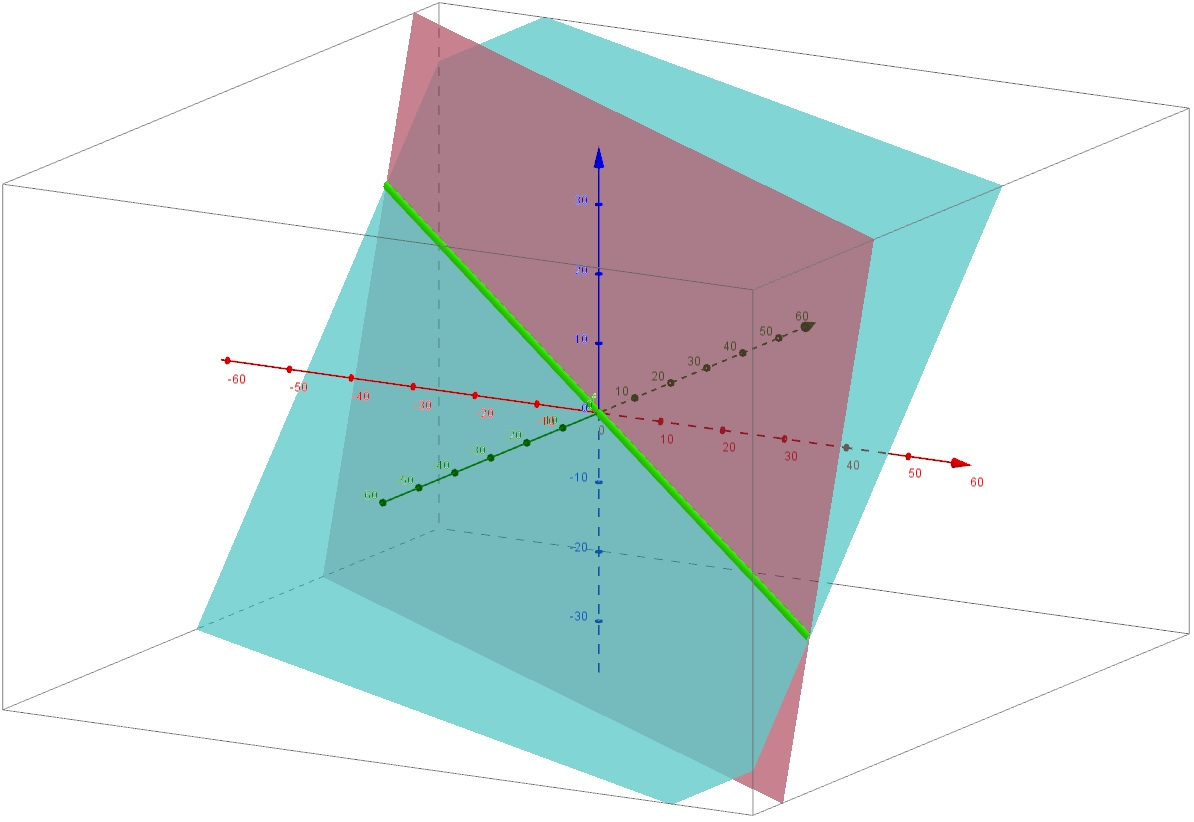
\includegraphics[width = 0.8\textwidth]{//home/the-scientist/linear/linear-algebra/asg1/resources/sol_space_white.jpg}
        \end{figure}
        \\$\therefore P_1 \bigcap P_2$ = span \{$(-4, 3, 1)$\}
\end{proof}
\end{document}
